\chapter{A Theoretical Overview}
\label{chap:theorysection}

Within this chapter, a brief introduction and background to the \ac{SM} is given. Its success as a rigorously tested and widely accepted theory is discussed as are it's deficiencies, leading to the argument that this theory is not a complete description of our universe. The motivations for new physics at the \TeV scale and in particular Supersymmetric theories are outlined within Section (\ref{sec:susytheory}), with the chapter concluding with how an experimental signature of such theories can be produced and observed at the \ac{lhc}, Section (\ref{sec:susysearches}).

\section{The Standard Model}

\label{sec:thesm}

The \ac{SM} is the name given to the relativistic  \acf{QFT}, where particles are represented as excitations of fields, which describe the interactions and properties of all the known elementary particles \cite{PhysRevLett.19.1264}\cite{Glashow:1961tr}\cite{Salam:1968rm}\cite{Hooft1971167}. It is a renormalisable field theory which contains three symmetries: $SU(3)$ for colour charge, SU(2) for weak isospin and U(1) relating to weak hyper charge, which require its Lagrangian \lsm to be invariant under local gauge transformation. 

Within the \ac{SM} theory, matter is composed of spin \half fermions, which interact with each other via the exchange of spin-1 gauge bosons. A summary of the known fundamental fermions and bosons is given in Table \ref{tab:sm_particles}.

\begin{table}[h!]
\footnotesize
\begin{center}
\begin{tabular*}{0.75\textwidth}{@{\extracolsep{\fill}}ccccc}
\hline
Particle                   & Symbol      & Spin & Charge         & Mass (\GeV) \\ 
\multicolumn{5}{c}{\textbf{First Generation Fermions}}  					 \\ \hline\hline
Electron Neutrino &$\nu_{e}$   & \half & 0                     &   $< 2.2 \times 10^{-6}$ \\ 
Electron                  & e                 & \half & -1                    &   $0.51 \times 10^{-3}$ \\ 
Up Quark                & u                 & \half & $\frac{2}{3}$ &   $2.3 ^{+0.7}_{-0.5} \times 10^{-3}$ \\ 
Down Quark          & d                 & \half & $-\frac{1}{3}$&   $4.8 ^{+0.7}_{-0.3}\times 10^{-3}$ \\ \cline{1-5}
\multicolumn{5}{c}{\textbf{Second Generation Fermions}}  					 \\ \hline\hline
Muon Neutrino       &$\nu_{\mu}$& \half & 0                     &   -                           \\ 
Muon                       & $\mu$       & \half & -1                    &   $1.05 \times 10^{-3}$ \\
Charm Quark        & c                 & \half & $\frac{2}{3}$ &   $1.275 \pm 0.025$ \\ 
Strange Quark      & s                 & \half & $-\frac{1}{3}$&   $95 \pm 5 \times 10^{-3}$ \\ \cline{1-5}
\multicolumn{5}{c}{\textbf{Third Generation Fermions}}  					 \\ \hline\hline
Tau Neutrino         &$\nu_{\tau}$& \half & 0                     &   -                           \\ 
Tau                          & $\tau$       & \half & -1                    &   1.77		 	\\ 
Top Quark              & t                 & \half & $\frac{2}{3}$ &   $173.5  \pm 0.8$ \\ 
Bottom Quark        & b                 & \half & $-\frac{1}{3}$&   $4.65  \pm 0.03$ \\ \cline{1-5}
\multicolumn{5}{c}{\textbf{Gauge Bosons}}  					 \\ \hline\hline
Photon                    &$\gamma$&1   & 0                         &   0                           \\ 
W Boson                 & $\Wboson$&1& $\pm$1              &   80.385 $\pm 0.015$ \\ 
Z Boson                 & $\Zboson$& 1 & 0		          &   $91.187  \pm 0.002$ \\ 
Gluons                   & g                 & 1 & 0			 &   0 \\ 
Higgs Boson         & H                & 0 & 0			 &   125.3 $\pm 0.5$ \cite{Chatrchyan:2012ufa} \\ 
\end{tabular*}
\end{center}
\caption[The fundamental particles of the \ac{SM}, with spin, charge and mass displayed.]{The fundamental particles of the \ac{SM}, with spin, charge and mass displayed. Latest mass measurements taken from \cite{pdg2012}. }
\label{tab:sm_particles}

\end{table}

Fermions are separated into quarks and leptons of which only quarks interact with the strong nuclear force. Quarks unlike leptons are not seen as free particles in nature, but rather exist only within baryons, composed of three quarks with an overall integer charge, and quark-anti-quark pairs called mesons. Both leptons and quarks are grouped into three generations which have the same properties, but with ascending mass in each subsequent generation. 

The gauge bosons mediate the interactions between fermions. The field theories of \acf{QED} and \acf{QCD}, yield massless mediator bosons, the photon and eight coloured gluons which are consequences of the gauge invariance of those theories, detailed in Section (\ref{subsec:gaugetheories}).  

The unification of the electromagnetic and weak-nuclear forces into the current Electroweak theory yield the weak gauge bosons, \Wboson and \Zboson through the mixing of the associated gauge fields. The force carriers of this theory were experimentally detected by the observation of weak neutral current, discovered in 1973 in the Gargamelle bubble chamber located at \ac{CERN} \cite{Hasert:1973ff}, with the masses of the weak gauge bosons measured by the UA1 and U2 experiments at the \acf{SPS} collider in 1983 \cite{Arnison:1983mk}\cite{Banner:1983jy}.

\subsection{Gauge Symmetries of the SM}

\label{subsec:gaugetheories}

Symmetries are of fundamental importance in the description of physical phenomena. Noether's theorem states that for a dynamical system, the consequence of any symmetry is an associated conserved quantity \cite{Noether1918}. Invariance under translations, rotations, and Lorentz transformations in physical systems lead to conservation of momentum, energy and angular momentum. 

In the \ac{SM}, a quantum theory described by Lagrangian formalism, the weak, strong and electromagnetic interactions are described in terms of ``gauge theories''.  A gauge theory possesses invariance under a set of ``local transformations", which are transformations whose parameters are space-time dependent. The requirement of gauge invariance within the \ac{SM} necessitates the introduction of force-mediating gauge bosons and interactions between fermions and the bosons themselves. Given the nature of the topics covered by this thesis, the formulation of \ac{EWK}  within the \ac{SM} Lagrangian is reviewed within this section.

The simplest example of the application of the principle of local gauge invariance within the \ac{SM} is in \acf{QED}, the consequences of which require a massless photon field \cite{quarksandleptons}\cite{introtoparticles}. 

Starting from the free Dirac Lagrangian written as 

\begin{equation}
\label{eq:diracequation}
\mathcal{L} = \bar{\psi}(i\gamma^{\mu}\partial_{\mu} - m)\psi,
\end{equation}

where \fermfield represents a free non interacting fermionic field, with the matrices $\gamma^{\mu}$, $\mu \in  0,1,2,3$ defined by the anti commutator relationship $\gamma^{\mu}\gamma^{\nu}  + \gamma^{\mu}\gamma^{\nu} = 2\eta^{\mu\nu}I_{4}$, with $\eta^{\mu\nu}$ being the flat space-time metric $(+,-,-,-)$, and $I_{4}$ the 4 $\times$ 4 identity matrix. 

Under a local U(1) abelian gauge transformation in which \fermfield transforms as:

\begin{equation}
\fermfield(x) \rightarrow \fermfield^{'}(x) = e^{i\theta(x)}\fermfield(x) \qquad      \bar{\fermfield}(x) \rightarrow \bar{\fermfield}^{'}(x) = e^{i\theta(x)}\bar{\fermfield}(x)
\end{equation}

the kinetic term of the Lagrangian will not remain invariant, due to the partial derivative interposed between the $\bar{\fermfield}$ and \fermfield yielding,

\begin{equation}
\label{eq:remainderterm}
\partial_{\mu}\fermfield \rightarrow  e^{i\theta(x)}\partial_{\mu}\fermfield + ie^{i\theta(x)}\fermfield\partial_{\mu}\theta.
\end{equation} 

To ensure that $\mathcal{L}$ remains invariant, a modified derivative, $D_{\mu}$, that transforms covariantly under phase transformations is introduced. In doing this a vector field $A_{\mu}$ with transformation properties that cancel out the unwanted term in (\ref{eq:remainderterm}) must also be included, 

\begin{equation}
\label{eq:afieldtrans}
D_{\mu} \equiv \partial_{\mu} - ieA_{\mu},   \qquad A_{\mu} \rightarrow A_{\mu} + \frac{1}{e}\partial_{\mu}\theta .
\end{equation}

Invariance of the Lagrangian is then achieved by replacing $\partial_{\mu}$ by $D_{\mu}$:

\begin{align}
\label{eq:covlag}
\mathcal{L} &= i\bar{\fermfield}\gamma^{\mu}D_{\mu}\fermfield - m\bar{\fermfield}\fermfield \nonumber    \\
 &= \bar{\fermfield}(i\gamma^{\mu}\partial_{\mu} - m)\fermfield +  e\bar{\fermfield}\gamma^{\mu}\fermfield A_{\mu}
\end{align}


An additional interaction term is now present in the Lagrangian, coupling the Dirac particle to this vector field, which is interpreted as the photon in \ac{QED}. To regard this new field as the physical photon field, a term corresponding to its kinetic energy must be added to the Lagrangian from Equation (\ref{eq:covlag}). Since this term must also be invariant under the conditions of Equation (\ref{eq:afieldtrans}), it is defined in the form $F_{\mu\nu} = \partial^{\mu}A^{\nu} - \partial_{\nu}A_{\mu}$. 

This then leads to the Lagrangian of \ac{QED}: 

\begin{equation}
\label{qedlagrangian}
\mathcal{L}_{QED} =.\overbrace{i\bar{\fermfield}\gamma^{\mu}\partial_{\mu}\fermfield - \frac{1}{4}F_{\mu\nu}F^{\mu\nu} }^\text{kinetic term} + \overbrace{m\bar{\fermfield}\fermfield}^\text{mass term} + \overbrace{e\bar{\fermfield}\gamma^{\mu}\fermfield A_{\mu} }^\text{interaction term}
\end{equation}

Within the Lagrangian there remains no mass term of the form $m^{2}A_{\mu}A^{\mu}$, which is prohibited by gauge invariance. This implies that the gauge particle, the photon, must be massless.


\subsection{The Electroweak Sector and Electroweak Symmetry Breaking}

\label{subsec:ewsb}
The same application of gauge symmetry and the requirement of local gauge invariance can be used to unify \ac{QED} and the Weak force in the \acf{EWK}. The nature of \ac{EWK} interactions is encompassed within a Lagrangian invariant under transformations of the group $SU(2)_{L} \times U(1)_{Y}$. 

The weak interactions from experimental observation \cite{wu-parity}, are known to violate parity and are therefore not symmetric under interchange of left and right helicity fermions. Thus within the \ac{SM} the left and right handed parts of these fermion fields are treated separately. A fermion field is then split into two left and right handed chiral components, $\fermfield = \fermfield_{L} + \fermfield_{R}$, where $\fermfield_{L\slash R} = (1 \pm \gamma^{5})\fermfield$. 

The $SU(2)_{L}$ group is the special unitary group of $2 \times 2$ matrices $U$ satisfying $UU^{\dagger} = I$ and det(U) = 1. It may be written in the form $U = e^{-i\omega_{i}T_{i}}$, with the generators of the group $T_{i} = \frac{1}{2}\tau_{i}$ where $\tau_{i}$, $i \in$ 1,2,3 being the $2 \times 2$ Pauli matrices

\begin{equation}
\tau_{1}= \left( \begin{array}{ccc}
0 & 1\\
1 & 0\end{array} \right)\qquad
\tau_{2}= \left( \begin{array}{ccc}
0 & -i\\
i & 0\end{array} \right)\qquad
\tau_{3}= \left( \begin{array}{ccc}
1 & 0\\
0 & -1\end{array} \right),
\end{equation}


which form a non Abelian group obeying the commutation relation $[T^{a},T^{b}] \equiv  if^{abc}T^{c} \neq 0$. The gauge fields that accompany this group are represented by $\hat{W}_{\mu}  = (\hat{W}^{1}_{\mu},\hat{W}^{2}_{\mu},\hat{W}^{3}_{\mu}$  ) and act only on the left handed component of the fermion field $\fermfield_{L}$.

One additional generator $Y$ which represents the hypercharge of the particle under consideration is introduced through the $U(1)_{Y}$ group acting on both components of the fermion field, with an associated vector boson field $\hat{B}_{\mu}$.  

The $SU(2)_{L} \times U(1)_{Y}$ transformations of the left and right handed components of $\fermfield$ are summarised by,

\begin{align}
\label{eq:su2xu1transform}
 & \chi_{L} \rightarrow \chi^{'}_{L} = e^{i\theta(x) \cdot T + i\theta(x)Y}\chi_{L}, \nonumber \\
 & \fermfield_{R} \rightarrow \fermfield^{'}_{R} = e^{i\theta(x)Y}\fermfield_{R}, 
\end{align}

where the left handed fermions form isospin doubles $\chi_{L}$ and the right handed fermions are isosinglets $\fermfield_{R}$. For the first generation of leptons and quarks this represents

\begin{align}
\label{firstdoublet}
 \chi_{L} &= \left( \begin{array}{c} 
\nu_{e} \\
e \end{array} \right)_{L}, \qquad
 \left( \begin{array}{c} 
u  \\
d \end{array} \right)_{L}, \nonumber \\
 \fermfield_{R} &= e_{R}, \qquad \qquad \qquad u_{R}, d_{R}.
\end{align}

Imposing local gauge invariance within $\mathcal{L}_{EWK}$ is once again achieved by modifying the covariant derivative

\begin{equation}
\label{covderivative}
D_{\mu} = \partial_{\mu} - \frac{ig}{2}\tau^{i}W^{i}_{\mu} - \frac{ig^{'}}{2}Y B_{\mu},
\end{equation}

where $g$ and $g^{'}$ are the coupling constant of the $SU(2)_{L}$ and $U(1)_{Y}$ groups respectively. Taking the example of the first generation of fermions defined in Equation.(\ref{firstdoublet}), with input hypercharge values of -1 and -2 for $\chi_{L}$ and $e_{R}$ respectively, would lead to a Lagrangian $\mathcal{L}_{1}$ of the form,

\begin{align}
 \label{ewklagrangian}
\mathcal{L}_{1} =  &\bar{\chi}_{L}\gamma^{\mu}\lbrack i\partial_{\mu} - g\frac{1}{2}\tau\cdot W_{\mu} - g^{'}(-\frac{1}{2})B_{\mu} \rbrack\chi_{L} \nonumber \\
& + \bar{e}_{R}\gamma^{\mu}\lbrack i\partial_{\mu} - g^{'}(-1)B_{\mu}\rbrack e_{R} - \frac{1}{4}W_{\mu\nu}\cdot W^{\mu\nu} - \frac{1}{4}B_{\mu\nu}B^{\mu\nu}.
\end{align}

As in \ac{QED}, these additional gauge fields introduce field strength tensors $B_{\mu\nu}$ and $W_{\mu\nu}$,

\begin{align}
\hat{B}_{\mu\nu} &=  \partial_{\mu}\hat{B}_{\nu} - \partial_{\nu}\hat{B}_{\mu} \\
\hat{W}_{\mu\nu} &=  \partial_{\mu}\hat{W}_{\nu} - \partial_{\nu}\hat{W}_{\mu} - g\hat{W}_{\mu}\times\hat{W}_{\mu}
\end{align}

corresponding to the kinetic energy and self coupling of the $W_{\mu}$ fields and the kinetic energy term of the $B_{\mu}$ field.

None of these gauge bosons are physical particles, and instead linear combinations of these gauge bosons make up $\gamma$ and the W and Z bosons, defined as 

\begin{equation}
\label{bosonrotations}
W^{\pm} = \frac{1}{\sqrt{2}} \left(W^{1}_{\mu} \mp iW^{2}_{\mu}\right), \qquad   
\left( \begin{array}{c} 
Z_{\mu} \\
A_{\mu} \end{array} \right)   = 
\left( \begin{array}{cc} 
cos\theta_{W} & -sin\theta_{W} \\
sin\theta_{W} & cos\theta_{W} \end{array} \right) 
\left( \begin{array}{c} 
W^{3}_{\mu} \\
B_{\mu} \end{array} \right),
\end{equation}

where the mixing angle, $\theta_{w} = \tan ^{-1} \frac{g^{'}}{g}$, relates the coupling of the neutral weak and electromagnetic interactions. 

As in the case of the formulation of the \ac{QED} Lagrangian there remains no mass term for the photon. However this is also the case for the W, Z and fermions in the Lagrangian, contrary to experimental measurement. Any explicit introduction of mass terms would break the symmetry of the Lagrangian and instead mass terms can be introduced through spontaneous breaking of the \ac{EWK} symmetry via the Higgs mechanism.

The Higgs mechanism induces spontaneous symmetry breaking through the introduction of a complex scalar SU(2) doublet field $\phi$ which attains a non-zero \acf{VEV} \cite{higgs1}\cite{higgs2}\cite{higgs3}\cite{higgs4}. 

\begin{equation}
\phi =  \left( \begin{array}{c} 
\phi^{+} \\
\phi^{0} \end{array} \right)  \qquad with \qquad
\begin{array}{c} 
\phi^{+} \equiv  (\phi_{1} + i\phi_{2})/\sqrt{2}\\
\phi^{0} \equiv (\phi_{3}+i\phi_{4})/\sqrt{2} \end{array} 
\end{equation}

The Lagrangian defined in Equation (\ref{ewklagrangian}) attains an additional term $\mathcal{L}_{Higgs}$ of the form 

\begin{align}
\label{higgslagrangian}
\mathcal{L}_{Higgs} &= \overbrace{(D_{\mu}\phi)^{\dagger}(D^{\mu}\phi)}^\text{kinetic} - \overbrace{\mu^{2}\phi^{\dagger}\phi - \lambda(\phi^{\dagger}\phi)^{2}}^\text{potential V(\phi)} \qquad (\mu^{2},\lambda) > 0 \in \mathbb{R}, \nonumber \\
\mathcal{L}_{SM} &= \mathcal{L}_{EWK} + \mathcal{L}_{Higgs},
\end{align}

where the covariant derivative $D_{\mu}$ is that defined in Equation (\ref{covderivative}). The last two terms of $\mathcal{L}_{Higgs}$ correspond to the Higgs potential, in which real positive values of $\mu^{2}$ and $\lambda$ are required to ensure the generation of masses for the bosons and leptons. The minimum of this potential is found at $\phi^{\dagger}\phi = \frac{1}{2}(\phi^{2}_{1}+\phi^{2}_{2}+\phi^{2}_{3} + \phi^{2}_{4}) =\mu^{2} / \lambda = v^{2}$, where $v$ represents the \ac{VEV}.

Defining the ground state of the \phi field to be consistent with the $V(\phi)$ minimum, and then expanding around a ground state chosen to maintain an unbroken electromagnetic symmetry thus preserving a zero photon mass \cite{weinberghiggs} leads to

\begin{equation}
\phi_{0} =  \sqrt{\frac{1}{2}}\left( \begin{array}{c} 
0 \\
v  \end{array} \right) ,  \qquad \qquad 
\phi(x) =  e^{i\tau\cdot\theta(x)/v}\sqrt{\frac{1}{2}} \left( \begin{array}{c} 
0 \\
v +h(x)  \end{array} \right) , 
\end{equation} 

where the fluctuations from the vacuum $\phi_{0}$ are parametrized in terms of four real fields, $ \theta_{1},\theta_{2},\theta_{3}$ and $h(x)$. 

Choosing to gauge away the three massless Goldstone boson fields by setting $\theta(x)$ to zero and substituting $\phi(x)$ back into kinetic term of $\mathcal{L}_{Higgs}$ from Equation (\ref{higgslagrangian}) leads to mass terms for the $W^{\pm}$ and Z bosons

\begin{equation}
(D_{\mu}\phi)^{\dagger}(D^{\mu}\phi) = \frac{1}{2}(\partial_{\mu}h)^{2}+\frac{g^{2}v^{2}}{2}W^{+}_{\mu}W^{-\mu} + \frac{v^{2}g^{2}}{8\cos^{2}\theta_{w}}Z_{\mu}Z^{\mu}+0A_{\mu}A^{\mu}  ,
\end{equation}

where the relations between the physical and electroweak gauge fields from Equation (\ref{bosonrotations}) are used. The $W^{\pm}$ and $Z$ boson masses can then be determined to be

\begin{equation}
M_{W} = \frac{1}{2}gv \qquad M_{Z} = \frac{1}{2}\frac{gv}{\cos\theta_{w}}.
\end{equation}

This mechanism is also used to generate fermion masses by introducing a Yukawa coupling between the fermions and the $\phi$ field \cite{Yukawa01011955}, with the coupling strength of a particle to the $\phi$ field governing its mass. Additionally a scalar boson h with mass $m_{h}=v\sqrt{\frac{\lambda}{2}}$, is also predicted as a result of this spontaneous symmetry breaking and became known as the Higgs boson. Its discovery by the \ac{CMS} and \ac{ATLAS} experiments in 2012 is the first direct evidence to support this method of mass generation within the \ac{SM}.

\section{Motivation for Physics Beyond the Standard Model}

\label{sec:bsmmotivation}

As has been described, the \ac{SM} has proven to be a very successful theory, predicting the existence of the \Wboson and \Zboson bosons and the top quark long before they were experimentally observed. However the theory does not accurately describe all observed phenomena and has some fundamental theoretical flaws that hint at the need for additional extensions to the current theory.

On a theoretical level, the \ac{SM} is unable to incorporate the gravitational interactions of fundamental particles within the theory. Whilst at the electroweak energy scales the relative strength of gravity is negligible compared to the other three fundamental forces, at much higher energy scales, $\text{M}_{\text{planck}} \sim 10^{18} \text{\GeV}$, quantum gravitational effects become increasingly dominant. The failure to reconcile gravity within the \ac{SM}, demonstrates that the \ac{SM} must become invalid at some higher energy scale. 

Other deficiencies with the \ac{SM} include the fact that the predicted rate of Charge-Parity violation does not account for the matter dominated universe which we inhabit, and that the \ac{SM} prediction of a massless neutrino conflicts with the observation of neutrino flavour mixing, attributed to mixing between neutrino mass eigenstates \cite{PhysRevLett.81.1562}\cite{BeckerSzendy:1992ym}. 

Perhaps one of the most glaring gaps in the predictive power of the \ac{SM} is that there exists no candidate to explain the cosmic dark matter observed in galactic structures through indirect techniques including gravitational lensing and measurement of the orbital velocity of stars at galactic edges. Any such candidate must be very weakly interacting but must also be stable, owing to the lack of direct detection of the decay products of such an process. Therefore a stable dark matter candidate, is one of the main obstacles to address for any \acf{BSM} physics model.

 The recent discovery of the Higgs boson whilst a significant victory for the predictive power of the \ac{SM}, brings with it still unresolved questions. This issue is commonly described as the ``hierarchy problem''. 
 
 In the absence of new physics between the \TeV and Planck scale, calculating beyond tree-level contributions to the Higgs mass term given by its self interaction, result in divergent terms that push the Higgs mass up to the planck mass $M_{planck}$. 
  
\begin{figure}[!h]
\centering
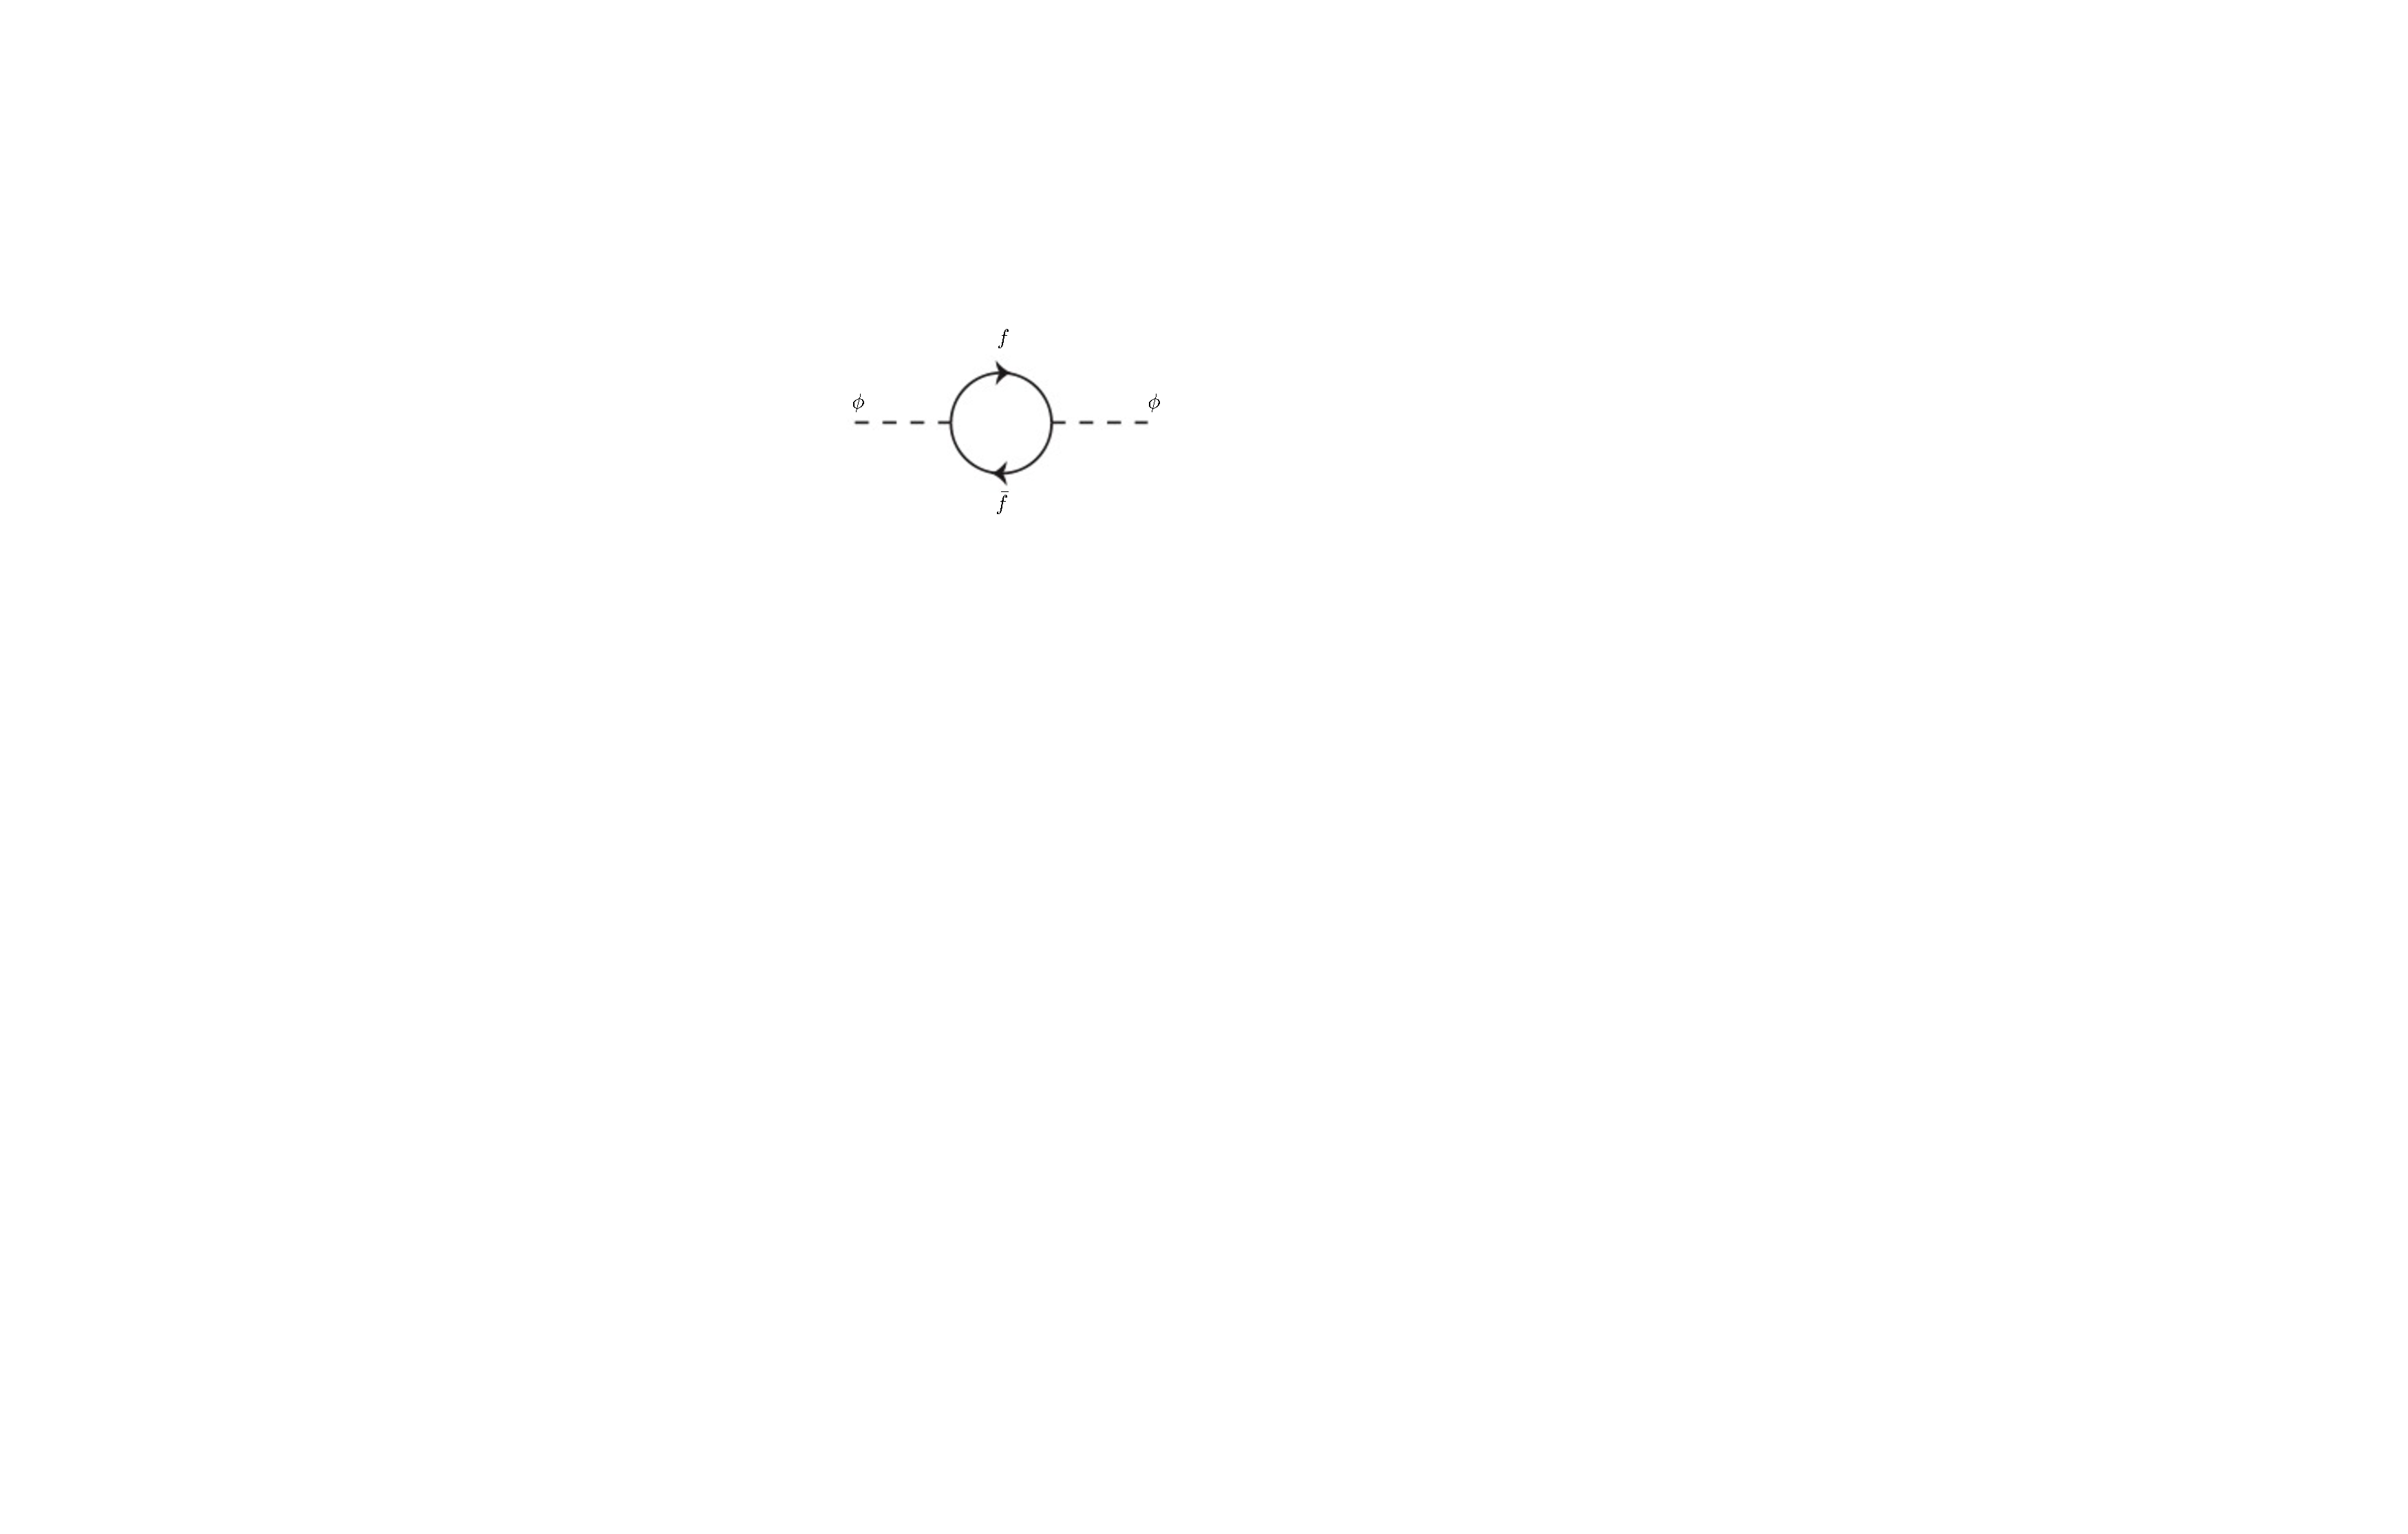
\includegraphics[width=0.45\textwidth]{plots/higgs_correction.pdf}
\caption[One loop quantum corrections to the Higgs squared mass parameter $m^{2}_{h}$ due to a fermion.]{One loop quantum corrections to the Higgs squared mass parameter $m^{2}_{h}$ due to a fermion.}  
\label{fig:higgscorrection}
\end{figure}

This can be demonstrated by considering the one loop quantum correction to the Higgs mass with a fermion f, shown in Figure \ref{fig:higgscorrection} with mass $m_{f}$. The Higgs field couples to f with a term in the Lagrangian $-\lambda_{f}h\bar{f}f$, yielding a correction of the form \cite{Martin:1997ns},
 
 \begin{equation}
 \delta m^{2}_{h} = -\frac{\lvert\lambda_{f}\rvert^{2}}{8\pi^{2}}\Lambda^{2} + �.. ,
 \end{equation}
 
 where $\lambda_{f}$ represents the coupling strength for each type of fermion $\propto m_{f}$, and $\Lambda$ the cutoff energy scale at which the \ac{SM} ceases to be a valid theory. 
 
 To recover the mass of the now discovered Higgs boson would require a fine-tuning of the parameters to cancel out these mass corrections of the Higgs mass to the scale of 30 orders of magnitude. This appears as an unnatural solution to physicists and it is this hierarchy problem that provides one of the strongest motivations for the theory of \acf{SUSY}.
 
\section{Supersymmmetry Overview}

\label{sec:susytheory}

Supersymmetry provides potential solutions to many of the issues raised in the previous section. It provides a dark matter candidate, can explain baryogenesis in the early universe and also provides an elegant solution to the hierarchy problem \cite{nilles1984supersymmetry}\cite{Haber:1984rc}\cite{Witten:1981nf}\cite{Wess197439}. At it's heart it represents a new space-time symmetry that relates fermions and bosons. This symmetry converts bosonic states into fermionic states, and vice versa, see Equation (\ref{susyoperator})  ,

\begin{equation}
\label{susyoperator}
Q \lvert \text{Boson}\rangle  = \lvert \text{Fermion}\rangle  \qquad Q \lvert \text{Fermion}\rangle = \lvert \text{Boson}\rangle,
\end{equation}
where the operator Q is the generator of these transformations. Quantum field theories which are invariant under such transformations are called supersymmetric.

This symmetry operator therefore acts upon a particles spin altering it by a half integer value. The consequences of the application of this additional space-time symmetry introduce a new rich phenomenology. For example in supersymmetric theories, both the left handed SU(2) doublet and right handed singlet of fermions will have a spin-0 superpartner, containing the same electric charge, weak isospin, and colour as its \ac{SM} partner. In the case of leptons $(\nu_{l},l)_{L}$, they will have two superpartners, a sneutrino $\widetilde{\nu_{l}}_{L}$ and a slepton $\widetilde{l}_{L}$, whilst the singlet $l_{R}$ also has a superpartner slepton $\widetilde{l}_{R}$. 
 
Each particle in a supersymmetric theory is paired together with their superpartners as a result of these supersymmetric transformations in a so called supermultiplet. These superpartners will then consequently also contribute to the corrections to the Higgs mass. Bosonic and fermionic loops contributing to the correction appear with opposite signs, and therefore cancellation of these divergent terms will stabilise the Higgs mass, solving the hierarchy problem \cite{muller2010introduction}\cite{aitchison2007supersymmetry}. 

One of the simplest forms of \ac{SUSY}, is to simply have a set of \ac{SM} supersymmetric partners with the same mass and interactions as their counterparts. However the current lack of any experimental evidence for that predicted sparticle spectrum implies \ac{SUSY} must be a broken symmetry in which any sparticle masses must be greater than their \ac{SM} counterparts.

There exist many techniques which can induce supersymmetric breaking \cite{Intriligator:2007zz}\cite{Shadmi:2006jv}\cite{Burgess:2006mn}. Of particular interest to experimental physicists are those at which the breaking scale is of an order that is experimentally accessible to the \ac{lhc} i.e. $\sim$ \TeV scale. Whilst there is no requirement for supersymmetric breaking to occur at this energy scale, for supersymmetry to provide a solution to the hierarchy problem, it is necessary for this scale to not differ too drastically from the \ac{EWK} scale \cite{Murayama:2007sy}\cite{baer2006weak}.

 
\subsection{R-Parity}

\label{subsec:rparity}

Some supersymmetric theories also present a solution to the dark matter problem. These theories contain a \acf{LSP}, which matches the criteria of a \acf{WIMP} required by cosmological observation when R-parity is conserved.  

Baryon (B) and Lepton (L) number conservation is forbidden in the \ac{SM} by renormalisability requirements. The violation of Baryon or Lepton number results in a proton lifetime much shorter than those set by experimental limits \cite{Martin:hep-ph9602349}. Another symmetry called R-parity is then often introduced to \ac{SUSY} theories to maintain baryon and lepton conservation. 

R-parity is described by the equation 

\begin{equation}
\label{eq:rparityequation}
R_{P} = (-1)^{3(B-L)+2s},
\end{equation}
where s represents the spin of the particles. $B =  \pm\frac{1}{3}$ for quarks/antiquarks and $B=0$ for all others, $L = \pm 1$ for leptons/antileptons, $L= 0$ for all others. 

R-parity ensures the stability of the proton in \ac{SUSY} models, and also has other consequences for the production and decay of supersymmetric particles. In particle colliders supersymmetric particles can only be pair produced, and similarly the decay of any produced supersymmetric particle is restricted to a \ac{SM} particle and a lighter supersymmetric particle as allowed by conservation laws. A further implication of R-parity is that once a supersymmetric particle has decayed to the \ac{LSP} it remains stable, unable to decay into a \ac{SM} particle.  

A \ac{LSP} will not interact in a detector at a particle collider, leaving behind a missing energy $\met$ signature. The assumption of R-parity and its consequences are used to determine the physical motivation and search strategies for \ac{SUSY} models at the \ac{lhc}. 

\section{Experimental Signatures of SUSY at the LHC}
\label{sec:susysearches}

Should strongly interacting sparticles be within the experimental reach of the \ac{lhc}, then it is expected that they can be produced in a variety of ways :

\begin{itemize}
\item squark/anti-squark and gluino pairs can be produced via both gluon fusion and quark/anti-quark scattering,
\item a gluino and squark produced together via quark-gluon scattering,
\item squark pairs produced via quark-quark scattering.
\end{itemize}

Whilst most \ac{SUSY} searches invoke the requirement of R-parity to explore parameter phase space, there still exist a whole plethora of possible \ac{SUSY} model topologies which could be waiting to be discovered at the \ac{lhc}. 

During the 2011 run period at $\com = 7$ \TeV, particular models were used to benchmark performance and experimental reach of both \ac{CMS} searches and previous experiments. The \acf{CMSSM} was initially chosen for a number of reasons \cite{Kane:1993td}, one of the most compelling being the reduction of the up to 105 new parameters that can be introduced by \ac{SUSY} (in addition to the existing 19 of the \ac{SM}), to just 5 free extra free parameters. It was this simplicity, combined with the theory not requiring any fine tuning of particle masses to produce experimentally verified \ac{SM} observables that made it an attractive model to interpret physics results. 

However recent results from the \ac{lhc} now strongly disfavour large swathes of \ac{CMSSM} parameter space \cite{Strege:2011pk}\cite{Citron:2012fg}\cite{Ghosh:2012dh}. In the face of such results a more pragmatic model independent search strategy is now applied across most \ac{SUSY} searches at the \ac{lhc}, see Section (\ref{subsec:sms}). 

As previously stated, a stable \ac{LSP} that exhibits the properties of a dark matter candidate would be weakly interacting and therefore will not be directly detected in a detector environment. Additionally the cascade decays of supersymmetric particles to this \ac{LSP} state would also result in significant hadronic activity. These signatures will then be characterised through large amounts of hadronic jets (see Section (\ref{subsec:cmsobjects-jets})), leptons and a significant amount of missing energy dependent upon the size of the mass splitting between the \ac{LSP} and the supersymmetric particle it has decayed from.

The \ac{SM} contains processes which can exhibit a similar event topology to that described above. The largest contribution coming from the general QCD environment of a hadron collider. A multitude of different analytical techniques are used by experimental physicists to reduce or estimate any reducible or irreducible backgrounds, allowing a possible \ac{SUSY} signature to be extracted. The techniques employed within this thesis are described in great detail within Section (\ref{sec:alphatintroduction}).

\subsection{Simplified models}

\label{subsec:sms}

With such a variety of different ways for a \ac{SUSY} signal to manifest itself, it is necessary to be able to interpret experimental reach through the masses of gluinos and squarks which can be excluded by experimental searches rather than on a model specific basis. 

This is accomplished through \ac{SMS} models, which are defined by a set of hypothetical particles and a sequence of their production and decay modes \cite{Alves:2011wf}\cite{Alwall:2008ag}. In the \ac{SMS} models considered within this thesis, only the production process for the two primary particles are considered. Each primary particle can undergo a direct or a cascade decay through an intermediate new particle. At the end of each decay chain there remains a neutral, undetected \ac{LSP} particle, denoted $\widetilde{\chi}_{LSP}$ which can represent a neutralino or gravitino. Essentially it is easier to consider each \ac{SMS} with branching ratios set to $100\%$. The masses of the primary particle and the \ac{LSP} remain as free parameters, in which the absolute value and relative difference between the primary and \ac{LSP} particle alter the kinematics of the event.

Different \ac{SMS} models are denoted with a T-prefix, with a summary of the types interpreted within this thesis listed below \cite{Chatrchyan:2013sza}.

\begin{itemize}
\item \textbf{T1,T1xxxx}, models represent a simplified version of gluino pair production with each gluino (superpartner to the gluon) undergoing a three-body decay to a quark-antiquark pair and the \ac{LSP} (i.e. $\widetilde{g} \rightarrow q\bar{q}\widetilde{\chi}_{LSP}$). The resultant final state from this decay is typically 4 jets + $\met$ in the absence of initial/final state radiation and detector effects. xxxx denotes models in which the quarks are of a specific flavour, typically t or b quark-antiquarks. 
\item \textbf{T2,T2xx}, models represent a simplified version of squark anti-squark production with each squark undergoing a two-body decay into a light-flavour quark and \ac{LSP} (i.e. $\widetilde{q} \rightarrow q\widetilde{\chi}_{LSP}$). This results in final states with less jets than gluino mediated production, typically 2 jets + $\met$ when again ignoring the effect of initial/final state radiation and detector effects. xx models represent decays in which both the quark and the squark within the decay is of a specific flavour, which in this thesis are again $\widetilde{t}$/t or $\widetilde{b}$/b.  

\end{itemize}

Models rich in b and t quarks are interpreted within this thesis as they remain of particular interest within ``Natural \ac{SUSY}'' scenarios \cite{Hisano:2000wy}\cite{Papucci:2011wy}. The largest contribution to the quadratic divergence in the Higgs mass parameter comes from a loop of top quarks via the Yukawa coupling. Cancellation of these divergences can be achieved in supersymmetric theories by requiring a light right handed top squark, $\widetilde{t}_{R}$, and left-handed double $SU(2)_{L}$ doublet containing top and bottom squarks, $(\frac{\widetilde{t}}{\widetilde{b}})_{L}$ \cite{Allanach:2012vj}. 

These theories therefore solve the hierarchy problem by predicting light $\sim$ \ac{EWK} scale third generation sleptons, to be accessible at the \ac{lhc}. Search strategies involving the requirement of b-tagging (see Section (\ref{subsec:cmsobjects-btagging})) are used to give sensitivity to these type of \ac{SUSY} scenarios and are discussed in greater detail within Chapter \ref{chap:SUSYsearches}.
 
Two example decay chains are shown in Figure \ref{fig:susydecayexamples}; the pair production of gluinos (\texttt{T1}) and the pair production of squarks (\texttt{T2}) decaying into \ac{SM} particles and \ac{LSP}'s.

\begin{figure}[ht]
\centering
\begin{minipage}[b]{0.45 \linewidth}
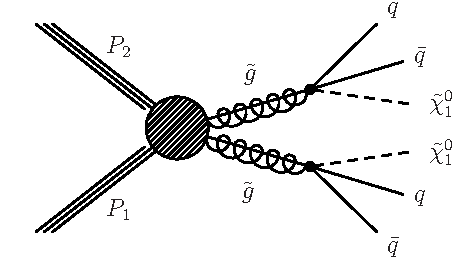
\includegraphics[width = 1.0\linewidth]{plots/t1susydecay.pdf}
\end{minipage}
\quad
\begin{minipage}[b]{0.45\linewidth}
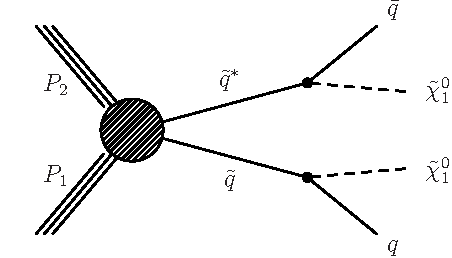
\includegraphics[width = 1.0\linewidth]{plots/t2susydecay.pdf}
\end{minipage}
\caption[Two example simplified model decay chains.]{Two example \ac{SMS} model decays (\texttt{T1} (left),\texttt{T2} (right)), which are used in interpretations of physics reach by \ac{CMS}. }
\label{fig:susydecayexamples}
\end{figure}


